\subsection{Boss and stealing employee}

\paragraph{Answers}
\subsubsection{Analyse this game using backward induction.}
\begin{figure}[ht]
    \centering
    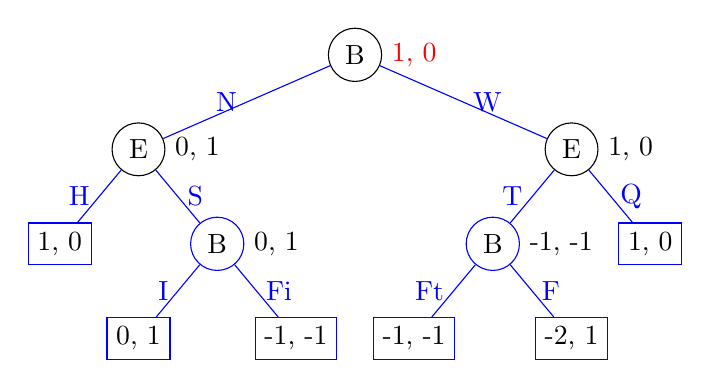
\begin{tikzpicture}[
        grow                    = down,
        % sibling distance        = 10em,
        level 1/.style          = {sibling distance=5.5cm},
        level 2/.style          = {sibling distance=2cm},
        level 3/.style          = {sibling distance=2cm},
        level distance          = 1.2cm,
        edge from parent/.style = {draw, edge from parent path={(\tikzparentnode) -- (\tikzchildnode)}},
        %sloped
      ]
        \node[circle, black,draw, label={[red]right: 1, 0}] {B}
            child {
                node[circle, draw, label={[black]right: 0, 1}] {E}
                child{
                        node[draw] {1, 0} 
                        edge from parent [left, blue] node {H}
                    }
                child {
                    node[circle, draw, label={[black]right: 0, 1}] {B}
                    child{
                        node[draw] {0, 1}
                        edge from parent [left, blue] node {I}
                    }
                    child{
                        node[draw] {-1, -1}
                        edge from parent [right, blue] node {Fi}
                    }
                    edge from parent [right, blue] node {S}
                }
                edge from parent [left, blue] node {N}
            }
            child {
                node[circle, black, draw, label={right: 1, 0}] {E}
                child {
                    node[circle, draw, label={[black]right: -1, -1}] {B}
                    child {
                        node [draw] {-1, -1}
                        edge from parent [left, blue] node {Ft}
                    }
                    child {
                        node [draw] {-2, 1}
                        edge from parent [right, blue] node {F}
                    }
                    edge from parent [left, blue] node {T}
                }
                child {
                    node [draw] {1, 0}
                    edge from parent [right, blue] node {Q}
                }
                edge from parent [right, blue] node {W}
            };
    \end{tikzpicture}
\end{figure}
The backwards induction shows, that the rational move for the Boss would be to give a warning
and then for the employee to quit steeling.

\subsubsection{What are the pure actions for the two players (boss and employee)? Construct the normal
form matrix.}

\subsubsection{Use this matrix to identify all the pure Nash equilibria of the normal form game.}

\subsubsection{Determine the subgame-perfect equilibrium (equilibria?) by eliminating all the Nash equi-
libria that fail to induce a NE in subgame}

\subsubsection{Compare to the solution based on backward induction.}